% Created by tikzDevice version 0.12.3.1 on 2021-10-13 07:12:56
% !TEX encoding = UTF-8 Unicode
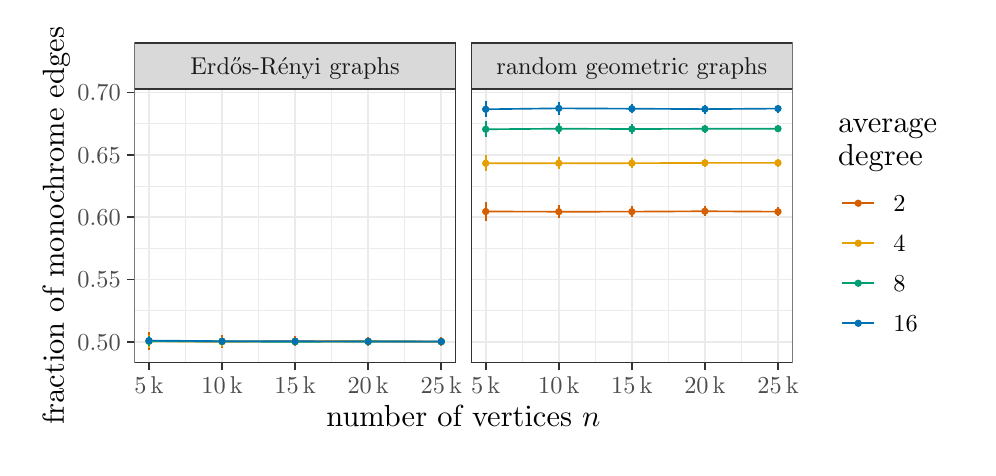
\begin{tikzpicture}[x=1pt,y=1pt]
\definecolor{fillColor}{RGB}{255,255,255}
\path[use as bounding box,fill=fillColor,fill opacity=0.00] (0,0) rectangle (339.67,151.77);
\begin{scope}
\path[clip] (  0.00,  0.00) rectangle (339.67,151.77);
\definecolor{drawColor}{RGB}{255,255,255}
\definecolor{fillColor}{RGB}{255,255,255}

\path[draw=drawColor,line width= 0.6pt,line join=round,line cap=round,fill=fillColor] (  0.00,  0.00) rectangle (339.67,151.77);
\end{scope}
\begin{scope}
\path[clip] ( 38.56, 30.69) rectangle (154.73,129.70);
\definecolor{fillColor}{RGB}{255,255,255}

\path[fill=fillColor] ( 38.56, 30.69) rectangle (154.73,129.70);
\definecolor{drawColor}{gray}{0.92}

\path[draw=drawColor,line width= 0.3pt,line join=round] ( 38.56, 49.56) --
	(154.73, 49.56);

\path[draw=drawColor,line width= 0.3pt,line join=round] ( 38.56, 72.07) --
	(154.73, 72.07);

\path[draw=drawColor,line width= 0.3pt,line join=round] ( 38.56, 94.57) --
	(154.73, 94.57);

\path[draw=drawColor,line width= 0.3pt,line join=round] ( 38.56,117.08) --
	(154.73,117.08);

\path[draw=drawColor,line width= 0.3pt,line join=round] ( 57.04, 30.69) --
	( 57.04,129.70);

\path[draw=drawColor,line width= 0.3pt,line join=round] ( 83.44, 30.69) --
	( 83.44,129.70);

\path[draw=drawColor,line width= 0.3pt,line join=round] (109.84, 30.69) --
	(109.84,129.70);

\path[draw=drawColor,line width= 0.3pt,line join=round] (136.24, 30.69) --
	(136.24,129.70);

\path[draw=drawColor,line width= 0.6pt,line join=round] ( 38.56, 38.30) --
	(154.73, 38.30);

\path[draw=drawColor,line width= 0.6pt,line join=round] ( 38.56, 60.81) --
	(154.73, 60.81);

\path[draw=drawColor,line width= 0.6pt,line join=round] ( 38.56, 83.32) --
	(154.73, 83.32);

\path[draw=drawColor,line width= 0.6pt,line join=round] ( 38.56,105.83) --
	(154.73,105.83);

\path[draw=drawColor,line width= 0.6pt,line join=round] ( 38.56,128.34) --
	(154.73,128.34);

\path[draw=drawColor,line width= 0.6pt,line join=round] ( 43.84, 30.69) --
	( 43.84,129.70);

\path[draw=drawColor,line width= 0.6pt,line join=round] ( 70.24, 30.69) --
	( 70.24,129.70);

\path[draw=drawColor,line width= 0.6pt,line join=round] ( 96.64, 30.69) --
	( 96.64,129.70);

\path[draw=drawColor,line width= 0.6pt,line join=round] (123.04, 30.69) --
	(123.04,129.70);

\path[draw=drawColor,line width= 0.6pt,line join=round] (149.45, 30.69) --
	(149.45,129.70);
\definecolor{drawColor}{RGB}{213,94,0}

\path[draw=drawColor,line width= 0.6pt,line join=round] ( 43.84, 41.84) --
	( 43.84, 41.84);

\path[draw=drawColor,line width= 0.6pt,line join=round] ( 43.84, 41.84) --
	( 43.84, 35.19);

\path[draw=drawColor,line width= 0.6pt,line join=round] ( 43.84, 35.19) --
	( 43.84, 35.19);

\path[draw=drawColor,line width= 0.6pt,line join=round] ( 70.24, 40.67) --
	( 70.24, 40.67);

\path[draw=drawColor,line width= 0.6pt,line join=round] ( 70.24, 40.67) --
	( 70.24, 36.19);

\path[draw=drawColor,line width= 0.6pt,line join=round] ( 70.24, 36.19) --
	( 70.24, 36.19);

\path[draw=drawColor,line width= 0.6pt,line join=round] ( 96.64, 40.42) --
	( 96.64, 40.42);

\path[draw=drawColor,line width= 0.6pt,line join=round] ( 96.64, 40.42) --
	( 96.64, 36.65);

\path[draw=drawColor,line width= 0.6pt,line join=round] ( 96.64, 36.65) --
	( 96.64, 36.65);

\path[draw=drawColor,line width= 0.6pt,line join=round] (123.04, 40.11) --
	(123.04, 40.11);

\path[draw=drawColor,line width= 0.6pt,line join=round] (123.04, 40.11) --
	(123.04, 36.80);

\path[draw=drawColor,line width= 0.6pt,line join=round] (123.04, 36.80) --
	(123.04, 36.80);

\path[draw=drawColor,line width= 0.6pt,line join=round] (149.45, 39.85) --
	(149.45, 39.85);

\path[draw=drawColor,line width= 0.6pt,line join=round] (149.45, 39.85) --
	(149.45, 36.74);

\path[draw=drawColor,line width= 0.6pt,line join=round] (149.45, 36.74) --
	(149.45, 36.74);
\definecolor{drawColor}{RGB}{230,159,0}

\path[draw=drawColor,line width= 0.6pt,line join=round] ( 43.84, 40.83) --
	( 43.84, 40.83);

\path[draw=drawColor,line width= 0.6pt,line join=round] ( 43.84, 40.83) --
	( 43.84, 36.13);

\path[draw=drawColor,line width= 0.6pt,line join=round] ( 43.84, 36.13) --
	( 43.84, 36.13);

\path[draw=drawColor,line width= 0.6pt,line join=round] ( 70.24, 40.15) --
	( 70.24, 40.15);

\path[draw=drawColor,line width= 0.6pt,line join=round] ( 70.24, 40.15) --
	( 70.24, 36.52);

\path[draw=drawColor,line width= 0.6pt,line join=round] ( 70.24, 36.52) --
	( 70.24, 36.52);

\path[draw=drawColor,line width= 0.6pt,line join=round] ( 96.64, 39.69) --
	( 96.64, 39.69);

\path[draw=drawColor,line width= 0.6pt,line join=round] ( 96.64, 39.69) --
	( 96.64, 36.94);

\path[draw=drawColor,line width= 0.6pt,line join=round] ( 96.64, 36.94) --
	( 96.64, 36.94);

\path[draw=drawColor,line width= 0.6pt,line join=round] (123.04, 39.60) --
	(123.04, 39.60);

\path[draw=drawColor,line width= 0.6pt,line join=round] (123.04, 39.60) --
	(123.04, 37.14);

\path[draw=drawColor,line width= 0.6pt,line join=round] (123.04, 37.14) --
	(123.04, 37.14);

\path[draw=drawColor,line width= 0.6pt,line join=round] (149.45, 39.48) --
	(149.45, 39.48);

\path[draw=drawColor,line width= 0.6pt,line join=round] (149.45, 39.48) --
	(149.45, 37.21);

\path[draw=drawColor,line width= 0.6pt,line join=round] (149.45, 37.21) --
	(149.45, 37.21);
\definecolor{drawColor}{RGB}{0,158,115}

\path[draw=drawColor,line width= 0.6pt,line join=round] ( 43.84, 40.24) --
	( 43.84, 40.24);

\path[draw=drawColor,line width= 0.6pt,line join=round] ( 43.84, 40.24) --
	( 43.84, 36.74);

\path[draw=drawColor,line width= 0.6pt,line join=round] ( 43.84, 36.74) --
	( 43.84, 36.74);

\path[draw=drawColor,line width= 0.6pt,line join=round] ( 70.24, 39.68) --
	( 70.24, 39.68);

\path[draw=drawColor,line width= 0.6pt,line join=round] ( 70.24, 39.68) --
	( 70.24, 37.02);

\path[draw=drawColor,line width= 0.6pt,line join=round] ( 70.24, 37.02) --
	( 70.24, 37.02);

\path[draw=drawColor,line width= 0.6pt,line join=round] ( 96.64, 39.38) --
	( 96.64, 39.38);

\path[draw=drawColor,line width= 0.6pt,line join=round] ( 96.64, 39.38) --
	( 96.64, 37.13);

\path[draw=drawColor,line width= 0.6pt,line join=round] ( 96.64, 37.13) --
	( 96.64, 37.13);

\path[draw=drawColor,line width= 0.6pt,line join=round] (123.04, 39.37) --
	(123.04, 39.37);

\path[draw=drawColor,line width= 0.6pt,line join=round] (123.04, 39.37) --
	(123.04, 37.43);

\path[draw=drawColor,line width= 0.6pt,line join=round] (123.04, 37.43) --
	(123.04, 37.43);

\path[draw=drawColor,line width= 0.6pt,line join=round] (149.45, 39.13) --
	(149.45, 39.13);

\path[draw=drawColor,line width= 0.6pt,line join=round] (149.45, 39.13) --
	(149.45, 37.45);

\path[draw=drawColor,line width= 0.6pt,line join=round] (149.45, 37.45) --
	(149.45, 37.45);
\definecolor{drawColor}{RGB}{0,114,178}

\path[draw=drawColor,line width= 0.6pt,line join=round] ( 43.84, 40.05) --
	( 43.84, 40.05);

\path[draw=drawColor,line width= 0.6pt,line join=round] ( 43.84, 40.05) --
	( 43.84, 37.27);

\path[draw=drawColor,line width= 0.6pt,line join=round] ( 43.84, 37.27) --
	( 43.84, 37.27);

\path[draw=drawColor,line width= 0.6pt,line join=round] ( 70.24, 39.45) --
	( 70.24, 39.45);

\path[draw=drawColor,line width= 0.6pt,line join=round] ( 70.24, 39.45) --
	( 70.24, 37.53);

\path[draw=drawColor,line width= 0.6pt,line join=round] ( 70.24, 37.53) --
	( 70.24, 37.53);

\path[draw=drawColor,line width= 0.6pt,line join=round] ( 96.64, 39.25) --
	( 96.64, 39.25);

\path[draw=drawColor,line width= 0.6pt,line join=round] ( 96.64, 39.25) --
	( 96.64, 37.73);

\path[draw=drawColor,line width= 0.6pt,line join=round] ( 96.64, 37.73) --
	( 96.64, 37.73);

\path[draw=drawColor,line width= 0.6pt,line join=round] (123.04, 39.03) --
	(123.04, 39.03);

\path[draw=drawColor,line width= 0.6pt,line join=round] (123.04, 39.03) --
	(123.04, 37.71);

\path[draw=drawColor,line width= 0.6pt,line join=round] (123.04, 37.71) --
	(123.04, 37.71);

\path[draw=drawColor,line width= 0.6pt,line join=round] (149.45, 38.95) --
	(149.45, 38.95);

\path[draw=drawColor,line width= 0.6pt,line join=round] (149.45, 38.95) --
	(149.45, 37.80);

\path[draw=drawColor,line width= 0.6pt,line join=round] (149.45, 37.80) --
	(149.45, 37.80);
\definecolor{drawColor}{RGB}{213,94,0}

\path[draw=drawColor,line width= 0.6pt,line join=round] ( 43.84, 38.53) --
	( 70.24, 38.35) --
	( 96.64, 38.49) --
	(123.04, 38.45) --
	(149.45, 38.30);
\definecolor{drawColor}{RGB}{230,159,0}

\path[draw=drawColor,line width= 0.6pt,line join=round] ( 43.84, 38.44) --
	( 70.24, 38.33) --
	( 96.64, 38.31) --
	(123.04, 38.36) --
	(149.45, 38.32);
\definecolor{drawColor}{RGB}{0,158,115}

\path[draw=drawColor,line width= 0.6pt,line join=round] ( 43.84, 38.46) --
	( 70.24, 38.36) --
	( 96.64, 38.26) --
	(123.04, 38.39) --
	(149.45, 38.31);
\definecolor{drawColor}{RGB}{0,114,178}

\path[draw=drawColor,line width= 0.6pt,line join=round] ( 43.84, 38.70) --
	( 70.24, 38.49) --
	( 96.64, 38.45) --
	(123.04, 38.37) --
	(149.45, 38.36);
\definecolor{drawColor}{RGB}{213,94,0}
\definecolor{fillColor}{RGB}{213,94,0}

\path[draw=drawColor,line width= 0.4pt,line join=round,line cap=round,fill=fillColor] ( 43.84, 38.53) circle (  1.11);

\path[draw=drawColor,line width= 0.4pt,line join=round,line cap=round,fill=fillColor] ( 70.24, 38.35) circle (  1.11);

\path[draw=drawColor,line width= 0.4pt,line join=round,line cap=round,fill=fillColor] ( 96.64, 38.49) circle (  1.11);

\path[draw=drawColor,line width= 0.4pt,line join=round,line cap=round,fill=fillColor] (123.04, 38.45) circle (  1.11);

\path[draw=drawColor,line width= 0.4pt,line join=round,line cap=round,fill=fillColor] (149.45, 38.30) circle (  1.11);
\definecolor{drawColor}{RGB}{230,159,0}
\definecolor{fillColor}{RGB}{230,159,0}

\path[draw=drawColor,line width= 0.4pt,line join=round,line cap=round,fill=fillColor] ( 43.84, 38.44) circle (  1.11);

\path[draw=drawColor,line width= 0.4pt,line join=round,line cap=round,fill=fillColor] ( 70.24, 38.33) circle (  1.11);

\path[draw=drawColor,line width= 0.4pt,line join=round,line cap=round,fill=fillColor] ( 96.64, 38.31) circle (  1.11);

\path[draw=drawColor,line width= 0.4pt,line join=round,line cap=round,fill=fillColor] (123.04, 38.36) circle (  1.11);

\path[draw=drawColor,line width= 0.4pt,line join=round,line cap=round,fill=fillColor] (149.45, 38.32) circle (  1.11);
\definecolor{drawColor}{RGB}{0,158,115}
\definecolor{fillColor}{RGB}{0,158,115}

\path[draw=drawColor,line width= 0.4pt,line join=round,line cap=round,fill=fillColor] ( 43.84, 38.46) circle (  1.11);

\path[draw=drawColor,line width= 0.4pt,line join=round,line cap=round,fill=fillColor] ( 70.24, 38.36) circle (  1.11);

\path[draw=drawColor,line width= 0.4pt,line join=round,line cap=round,fill=fillColor] ( 96.64, 38.26) circle (  1.11);

\path[draw=drawColor,line width= 0.4pt,line join=round,line cap=round,fill=fillColor] (123.04, 38.39) circle (  1.11);

\path[draw=drawColor,line width= 0.4pt,line join=round,line cap=round,fill=fillColor] (149.45, 38.31) circle (  1.11);
\definecolor{drawColor}{RGB}{0,114,178}
\definecolor{fillColor}{RGB}{0,114,178}

\path[draw=drawColor,line width= 0.4pt,line join=round,line cap=round,fill=fillColor] ( 43.84, 38.70) circle (  1.11);

\path[draw=drawColor,line width= 0.4pt,line join=round,line cap=round,fill=fillColor] ( 70.24, 38.49) circle (  1.11);

\path[draw=drawColor,line width= 0.4pt,line join=round,line cap=round,fill=fillColor] ( 96.64, 38.45) circle (  1.11);

\path[draw=drawColor,line width= 0.4pt,line join=round,line cap=round,fill=fillColor] (123.04, 38.37) circle (  1.11);

\path[draw=drawColor,line width= 0.4pt,line join=round,line cap=round,fill=fillColor] (149.45, 38.36) circle (  1.11);
\definecolor{drawColor}{gray}{0.20}

\path[draw=drawColor,line width= 0.6pt,line join=round,line cap=round] ( 38.56, 30.69) rectangle (154.73,129.70);
\end{scope}
\begin{scope}
\path[clip] (160.23, 30.69) rectangle (276.40,129.70);
\definecolor{fillColor}{RGB}{255,255,255}

\path[fill=fillColor] (160.23, 30.69) rectangle (276.40,129.70);
\definecolor{drawColor}{gray}{0.92}

\path[draw=drawColor,line width= 0.3pt,line join=round] (160.23, 49.56) --
	(276.40, 49.56);

\path[draw=drawColor,line width= 0.3pt,line join=round] (160.23, 72.07) --
	(276.40, 72.07);

\path[draw=drawColor,line width= 0.3pt,line join=round] (160.23, 94.57) --
	(276.40, 94.57);

\path[draw=drawColor,line width= 0.3pt,line join=round] (160.23,117.08) --
	(276.40,117.08);

\path[draw=drawColor,line width= 0.3pt,line join=round] (178.71, 30.69) --
	(178.71,129.70);

\path[draw=drawColor,line width= 0.3pt,line join=round] (205.11, 30.69) --
	(205.11,129.70);

\path[draw=drawColor,line width= 0.3pt,line join=round] (231.51, 30.69) --
	(231.51,129.70);

\path[draw=drawColor,line width= 0.3pt,line join=round] (257.92, 30.69) --
	(257.92,129.70);

\path[draw=drawColor,line width= 0.6pt,line join=round] (160.23, 38.30) --
	(276.40, 38.30);

\path[draw=drawColor,line width= 0.6pt,line join=round] (160.23, 60.81) --
	(276.40, 60.81);

\path[draw=drawColor,line width= 0.6pt,line join=round] (160.23, 83.32) --
	(276.40, 83.32);

\path[draw=drawColor,line width= 0.6pt,line join=round] (160.23,105.83) --
	(276.40,105.83);

\path[draw=drawColor,line width= 0.6pt,line join=round] (160.23,128.34) --
	(276.40,128.34);

\path[draw=drawColor,line width= 0.6pt,line join=round] (165.51, 30.69) --
	(165.51,129.70);

\path[draw=drawColor,line width= 0.6pt,line join=round] (191.91, 30.69) --
	(191.91,129.70);

\path[draw=drawColor,line width= 0.6pt,line join=round] (218.31, 30.69) --
	(218.31,129.70);

\path[draw=drawColor,line width= 0.6pt,line join=round] (244.71, 30.69) --
	(244.71,129.70);

\path[draw=drawColor,line width= 0.6pt,line join=round] (271.12, 30.69) --
	(271.12,129.70);
\definecolor{drawColor}{RGB}{213,94,0}

\path[draw=drawColor,line width= 0.6pt,line join=round] (165.51, 88.82) --
	(165.51, 88.82);

\path[draw=drawColor,line width= 0.6pt,line join=round] (165.51, 88.82) --
	(165.51, 81.79);

\path[draw=drawColor,line width= 0.6pt,line join=round] (165.51, 81.79) --
	(165.51, 81.79);

\path[draw=drawColor,line width= 0.6pt,line join=round] (191.91, 87.83) --
	(191.91, 87.83);

\path[draw=drawColor,line width= 0.6pt,line join=round] (191.91, 87.83) --
	(191.91, 82.96);

\path[draw=drawColor,line width= 0.6pt,line join=round] (191.91, 82.96) --
	(191.91, 82.96);

\path[draw=drawColor,line width= 0.6pt,line join=round] (218.31, 87.33) --
	(218.31, 87.33);

\path[draw=drawColor,line width= 0.6pt,line join=round] (218.31, 87.33) --
	(218.31, 83.26);

\path[draw=drawColor,line width= 0.6pt,line join=round] (218.31, 83.26) --
	(218.31, 83.26);

\path[draw=drawColor,line width= 0.6pt,line join=round] (244.71, 87.17) --
	(244.71, 87.17);

\path[draw=drawColor,line width= 0.6pt,line join=round] (244.71, 87.17) --
	(244.71, 83.74);

\path[draw=drawColor,line width= 0.6pt,line join=round] (244.71, 83.74) --
	(244.71, 83.74);

\path[draw=drawColor,line width= 0.6pt,line join=round] (271.12, 86.85) --
	(271.12, 86.85);

\path[draw=drawColor,line width= 0.6pt,line join=round] (271.12, 86.85) --
	(271.12, 83.70);

\path[draw=drawColor,line width= 0.6pt,line join=round] (271.12, 83.70) --
	(271.12, 83.70);
\definecolor{drawColor}{RGB}{230,159,0}

\path[draw=drawColor,line width= 0.6pt,line join=round] (165.51,105.91) --
	(165.51,105.91);

\path[draw=drawColor,line width= 0.6pt,line join=round] (165.51,105.91) --
	(165.51, 99.80);

\path[draw=drawColor,line width= 0.6pt,line join=round] (165.51, 99.80) --
	(165.51, 99.80);

\path[draw=drawColor,line width= 0.6pt,line join=round] (191.91,104.88) --
	(191.91,104.88);

\path[draw=drawColor,line width= 0.6pt,line join=round] (191.91,104.88) --
	(191.91,100.56);

\path[draw=drawColor,line width= 0.6pt,line join=round] (191.91,100.56) --
	(191.91,100.56);

\path[draw=drawColor,line width= 0.6pt,line join=round] (218.31,104.68) --
	(218.31,104.68);

\path[draw=drawColor,line width= 0.6pt,line join=round] (218.31,104.68) --
	(218.31,100.94);

\path[draw=drawColor,line width= 0.6pt,line join=round] (218.31,100.94) --
	(218.31,100.94);

\path[draw=drawColor,line width= 0.6pt,line join=round] (244.71,104.41) --
	(244.71,104.41);

\path[draw=drawColor,line width= 0.6pt,line join=round] (244.71,104.41) --
	(244.71,101.40);

\path[draw=drawColor,line width= 0.6pt,line join=round] (244.71,101.40) --
	(244.71,101.40);

\path[draw=drawColor,line width= 0.6pt,line join=round] (271.12,104.23) --
	(271.12,104.23);

\path[draw=drawColor,line width= 0.6pt,line join=round] (271.12,104.23) --
	(271.12,101.56);

\path[draw=drawColor,line width= 0.6pt,line join=round] (271.12,101.56) --
	(271.12,101.56);
\definecolor{drawColor}{RGB}{0,158,115}

\path[draw=drawColor,line width= 0.6pt,line join=round] (165.51,118.00) --
	(165.51,118.00);

\path[draw=drawColor,line width= 0.6pt,line join=round] (165.51,118.00) --
	(165.51,112.17);

\path[draw=drawColor,line width= 0.6pt,line join=round] (165.51,112.17) --
	(165.51,112.17);

\path[draw=drawColor,line width= 0.6pt,line join=round] (191.91,117.34) --
	(191.91,117.34);

\path[draw=drawColor,line width= 0.6pt,line join=round] (191.91,117.34) --
	(191.91,113.23);

\path[draw=drawColor,line width= 0.6pt,line join=round] (191.91,113.23) --
	(191.91,113.23);

\path[draw=drawColor,line width= 0.6pt,line join=round] (218.31,116.81) --
	(218.31,116.81);

\path[draw=drawColor,line width= 0.6pt,line join=round] (218.31,116.81) --
	(218.31,113.49);

\path[draw=drawColor,line width= 0.6pt,line join=round] (218.31,113.49) --
	(218.31,113.49);

\path[draw=drawColor,line width= 0.6pt,line join=round] (244.71,116.58) --
	(244.71,116.58);

\path[draw=drawColor,line width= 0.6pt,line join=round] (244.71,116.58) --
	(244.71,113.79);

\path[draw=drawColor,line width= 0.6pt,line join=round] (244.71,113.79) --
	(244.71,113.79);

\path[draw=drawColor,line width= 0.6pt,line join=round] (271.12,116.63) --
	(271.12,116.63);

\path[draw=drawColor,line width= 0.6pt,line join=round] (271.12,116.63) --
	(271.12,113.96);

\path[draw=drawColor,line width= 0.6pt,line join=round] (271.12,113.96) --
	(271.12,113.96);
\definecolor{drawColor}{RGB}{0,114,178}

\path[draw=drawColor,line width= 0.6pt,line join=round] (165.51,125.20) --
	(165.51,125.20);

\path[draw=drawColor,line width= 0.6pt,line join=round] (165.51,125.20) --
	(165.51,119.49);

\path[draw=drawColor,line width= 0.6pt,line join=round] (165.51,119.49) --
	(165.51,119.49);

\path[draw=drawColor,line width= 0.6pt,line join=round] (191.91,125.03) --
	(191.91,125.03);

\path[draw=drawColor,line width= 0.6pt,line join=round] (191.91,125.03) --
	(191.91,120.36);

\path[draw=drawColor,line width= 0.6pt,line join=round] (191.91,120.36) --
	(191.91,120.36);

\path[draw=drawColor,line width= 0.6pt,line join=round] (218.31,124.31) --
	(218.31,124.31);

\path[draw=drawColor,line width= 0.6pt,line join=round] (218.31,124.31) --
	(218.31,120.79);

\path[draw=drawColor,line width= 0.6pt,line join=round] (218.31,120.79) --
	(218.31,120.79);

\path[draw=drawColor,line width= 0.6pt,line join=round] (244.71,123.96) --
	(244.71,123.96);

\path[draw=drawColor,line width= 0.6pt,line join=round] (244.71,123.96) --
	(244.71,120.74);

\path[draw=drawColor,line width= 0.6pt,line join=round] (244.71,120.74) --
	(244.71,120.74);

\path[draw=drawColor,line width= 0.6pt,line join=round] (271.12,124.00) --
	(271.12,124.00);

\path[draw=drawColor,line width= 0.6pt,line join=round] (271.12,124.00) --
	(271.12,121.11);

\path[draw=drawColor,line width= 0.6pt,line join=round] (271.12,121.11) --
	(271.12,121.11);
\definecolor{drawColor}{RGB}{213,94,0}

\path[draw=drawColor,line width= 0.6pt,line join=round] (165.51, 85.34) --
	(191.91, 85.27) --
	(218.31, 85.29) --
	(244.71, 85.43) --
	(271.12, 85.28);
\definecolor{drawColor}{RGB}{230,159,0}

\path[draw=drawColor,line width= 0.6pt,line join=round] (165.51,102.77) --
	(191.91,102.79) --
	(218.31,102.80) --
	(244.71,102.90) --
	(271.12,102.92);
\definecolor{drawColor}{RGB}{0,158,115}

\path[draw=drawColor,line width= 0.6pt,line join=round] (165.51,115.06) --
	(191.91,115.26) --
	(218.31,115.15) --
	(244.71,115.23) --
	(271.12,115.27);
\definecolor{drawColor}{RGB}{0,114,178}

\path[draw=drawColor,line width= 0.6pt,line join=round] (165.51,122.29) --
	(191.91,122.62) --
	(218.31,122.49) --
	(244.71,122.34) --
	(271.12,122.53);
\definecolor{drawColor}{RGB}{213,94,0}
\definecolor{fillColor}{RGB}{213,94,0}

\path[draw=drawColor,line width= 0.4pt,line join=round,line cap=round,fill=fillColor] (165.51, 85.34) circle (  1.11);

\path[draw=drawColor,line width= 0.4pt,line join=round,line cap=round,fill=fillColor] (191.91, 85.27) circle (  1.11);

\path[draw=drawColor,line width= 0.4pt,line join=round,line cap=round,fill=fillColor] (218.31, 85.29) circle (  1.11);

\path[draw=drawColor,line width= 0.4pt,line join=round,line cap=round,fill=fillColor] (244.71, 85.43) circle (  1.11);

\path[draw=drawColor,line width= 0.4pt,line join=round,line cap=round,fill=fillColor] (271.12, 85.28) circle (  1.11);
\definecolor{drawColor}{RGB}{230,159,0}
\definecolor{fillColor}{RGB}{230,159,0}

\path[draw=drawColor,line width= 0.4pt,line join=round,line cap=round,fill=fillColor] (165.51,102.77) circle (  1.11);

\path[draw=drawColor,line width= 0.4pt,line join=round,line cap=round,fill=fillColor] (191.91,102.79) circle (  1.11);

\path[draw=drawColor,line width= 0.4pt,line join=round,line cap=round,fill=fillColor] (218.31,102.80) circle (  1.11);

\path[draw=drawColor,line width= 0.4pt,line join=round,line cap=round,fill=fillColor] (244.71,102.90) circle (  1.11);

\path[draw=drawColor,line width= 0.4pt,line join=round,line cap=round,fill=fillColor] (271.12,102.92) circle (  1.11);
\definecolor{drawColor}{RGB}{0,158,115}
\definecolor{fillColor}{RGB}{0,158,115}

\path[draw=drawColor,line width= 0.4pt,line join=round,line cap=round,fill=fillColor] (165.51,115.06) circle (  1.11);

\path[draw=drawColor,line width= 0.4pt,line join=round,line cap=round,fill=fillColor] (191.91,115.26) circle (  1.11);

\path[draw=drawColor,line width= 0.4pt,line join=round,line cap=round,fill=fillColor] (218.31,115.15) circle (  1.11);

\path[draw=drawColor,line width= 0.4pt,line join=round,line cap=round,fill=fillColor] (244.71,115.23) circle (  1.11);

\path[draw=drawColor,line width= 0.4pt,line join=round,line cap=round,fill=fillColor] (271.12,115.27) circle (  1.11);
\definecolor{drawColor}{RGB}{0,114,178}
\definecolor{fillColor}{RGB}{0,114,178}

\path[draw=drawColor,line width= 0.4pt,line join=round,line cap=round,fill=fillColor] (165.51,122.29) circle (  1.11);

\path[draw=drawColor,line width= 0.4pt,line join=round,line cap=round,fill=fillColor] (191.91,122.62) circle (  1.11);

\path[draw=drawColor,line width= 0.4pt,line join=round,line cap=round,fill=fillColor] (218.31,122.49) circle (  1.11);

\path[draw=drawColor,line width= 0.4pt,line join=round,line cap=round,fill=fillColor] (244.71,122.34) circle (  1.11);

\path[draw=drawColor,line width= 0.4pt,line join=round,line cap=round,fill=fillColor] (271.12,122.53) circle (  1.11);
\definecolor{drawColor}{gray}{0.20}

\path[draw=drawColor,line width= 0.6pt,line join=round,line cap=round] (160.23, 30.69) rectangle (276.40,129.70);
\end{scope}
\begin{scope}
\path[clip] ( 38.56,129.70) rectangle (154.73,146.27);
\definecolor{drawColor}{gray}{0.20}
\definecolor{fillColor}{gray}{0.85}

\path[draw=drawColor,line width= 0.6pt,line join=round,line cap=round,fill=fillColor] ( 38.56,129.70) rectangle (154.73,146.27);
\definecolor{drawColor}{gray}{0.10}

\node[text=drawColor,anchor=base,inner sep=0pt, outer sep=0pt, scale=  0.88] at ( 96.64,134.95) {Erd{\H o}s-R\'enyi graphs};
\end{scope}
\begin{scope}
\path[clip] (160.23,129.70) rectangle (276.40,146.27);
\definecolor{drawColor}{gray}{0.20}
\definecolor{fillColor}{gray}{0.85}

\path[draw=drawColor,line width= 0.6pt,line join=round,line cap=round,fill=fillColor] (160.23,129.70) rectangle (276.40,146.27);
\definecolor{drawColor}{gray}{0.10}

\node[text=drawColor,anchor=base,inner sep=0pt, outer sep=0pt, scale=  0.88] at (218.31,134.95) {random geometric graphs};
\end{scope}
\begin{scope}
\path[clip] (  0.00,  0.00) rectangle (339.67,151.77);
\definecolor{drawColor}{gray}{0.20}

\path[draw=drawColor,line width= 0.6pt,line join=round] ( 43.84, 27.94) --
	( 43.84, 30.69);

\path[draw=drawColor,line width= 0.6pt,line join=round] ( 70.24, 27.94) --
	( 70.24, 30.69);

\path[draw=drawColor,line width= 0.6pt,line join=round] ( 96.64, 27.94) --
	( 96.64, 30.69);

\path[draw=drawColor,line width= 0.6pt,line join=round] (123.04, 27.94) --
	(123.04, 30.69);

\path[draw=drawColor,line width= 0.6pt,line join=round] (149.45, 27.94) --
	(149.45, 30.69);
\end{scope}
\begin{scope}
\path[clip] (  0.00,  0.00) rectangle (339.67,151.77);
\definecolor{drawColor}{gray}{0.30}

\node[text=drawColor,anchor=base,inner sep=0pt, outer sep=0pt, scale=  0.88] at ( 43.84, 19.68) {5\,k};

\node[text=drawColor,anchor=base,inner sep=0pt, outer sep=0pt, scale=  0.88] at ( 70.24, 19.68) {10\,k};

\node[text=drawColor,anchor=base,inner sep=0pt, outer sep=0pt, scale=  0.88] at ( 96.64, 19.68) {15\,k};

\node[text=drawColor,anchor=base,inner sep=0pt, outer sep=0pt, scale=  0.88] at (123.04, 19.68) {20\,k};

\node[text=drawColor,anchor=base,inner sep=0pt, outer sep=0pt, scale=  0.88] at (149.45, 19.68) {25\,k};
\end{scope}
\begin{scope}
\path[clip] (  0.00,  0.00) rectangle (339.67,151.77);
\definecolor{drawColor}{gray}{0.20}

\path[draw=drawColor,line width= 0.6pt,line join=round] (165.51, 27.94) --
	(165.51, 30.69);

\path[draw=drawColor,line width= 0.6pt,line join=round] (191.91, 27.94) --
	(191.91, 30.69);

\path[draw=drawColor,line width= 0.6pt,line join=round] (218.31, 27.94) --
	(218.31, 30.69);

\path[draw=drawColor,line width= 0.6pt,line join=round] (244.71, 27.94) --
	(244.71, 30.69);

\path[draw=drawColor,line width= 0.6pt,line join=round] (271.12, 27.94) --
	(271.12, 30.69);
\end{scope}
\begin{scope}
\path[clip] (  0.00,  0.00) rectangle (339.67,151.77);
\definecolor{drawColor}{gray}{0.30}

\node[text=drawColor,anchor=base,inner sep=0pt, outer sep=0pt, scale=  0.88] at (165.51, 19.68) {5\,k};

\node[text=drawColor,anchor=base,inner sep=0pt, outer sep=0pt, scale=  0.88] at (191.91, 19.68) {10\,k};

\node[text=drawColor,anchor=base,inner sep=0pt, outer sep=0pt, scale=  0.88] at (218.31, 19.68) {15\,k};

\node[text=drawColor,anchor=base,inner sep=0pt, outer sep=0pt, scale=  0.88] at (244.71, 19.68) {20\,k};

\node[text=drawColor,anchor=base,inner sep=0pt, outer sep=0pt, scale=  0.88] at (271.12, 19.68) {25\,k};
\end{scope}
\begin{scope}
\path[clip] (  0.00,  0.00) rectangle (339.67,151.77);
\definecolor{drawColor}{gray}{0.30}

\node[text=drawColor,anchor=base east,inner sep=0pt, outer sep=0pt, scale=  0.88] at ( 33.61, 35.27) {0.50};

\node[text=drawColor,anchor=base east,inner sep=0pt, outer sep=0pt, scale=  0.88] at ( 33.61, 57.78) {0.55};

\node[text=drawColor,anchor=base east,inner sep=0pt, outer sep=0pt, scale=  0.88] at ( 33.61, 80.29) {0.60};

\node[text=drawColor,anchor=base east,inner sep=0pt, outer sep=0pt, scale=  0.88] at ( 33.61,102.80) {0.65};

\node[text=drawColor,anchor=base east,inner sep=0pt, outer sep=0pt, scale=  0.88] at ( 33.61,125.31) {0.70};
\end{scope}
\begin{scope}
\path[clip] (  0.00,  0.00) rectangle (339.67,151.77);
\definecolor{drawColor}{gray}{0.20}

\path[draw=drawColor,line width= 0.6pt,line join=round] ( 35.81, 38.30) --
	( 38.56, 38.30);

\path[draw=drawColor,line width= 0.6pt,line join=round] ( 35.81, 60.81) --
	( 38.56, 60.81);

\path[draw=drawColor,line width= 0.6pt,line join=round] ( 35.81, 83.32) --
	( 38.56, 83.32);

\path[draw=drawColor,line width= 0.6pt,line join=round] ( 35.81,105.83) --
	( 38.56,105.83);

\path[draw=drawColor,line width= 0.6pt,line join=round] ( 35.81,128.34) --
	( 38.56,128.34);
\end{scope}
\begin{scope}
\path[clip] (  0.00,  0.00) rectangle (339.67,151.77);
\definecolor{drawColor}{RGB}{0,0,0}

\node[text=drawColor,anchor=base,inner sep=0pt, outer sep=0pt, scale=  1.10] at (157.48,  7.64) {number of vertices $n$};
\end{scope}
\begin{scope}
\path[clip] (  0.00,  0.00) rectangle (339.67,151.77);
\definecolor{drawColor}{RGB}{0,0,0}

\node[text=drawColor,rotate= 90.00,anchor=base,inner sep=0pt, outer sep=0pt, scale=  1.10] at ( 13.08, 80.19) {fraction of monochrome edges};
\end{scope}
\begin{scope}
\path[clip] (  0.00,  0.00) rectangle (339.67,151.77);
\definecolor{fillColor}{RGB}{255,255,255}

\path[fill=fillColor] (287.40, 32.24) rectangle (334.17,128.15);
\end{scope}
\begin{scope}
\path[clip] (  0.00,  0.00) rectangle (339.67,151.77);
\definecolor{drawColor}{RGB}{0,0,0}

\node[text=drawColor,anchor=base west,inner sep=0pt, outer sep=0pt, scale=  1.10] at (292.90,114.00) {average};

\node[text=drawColor,anchor=base west,inner sep=0pt, outer sep=0pt, scale=  1.10] at (292.90,102.12) {degree};
\end{scope}
\begin{scope}
\path[clip] (  0.00,  0.00) rectangle (339.67,151.77);
\definecolor{fillColor}{RGB}{255,255,255}

\path[fill=fillColor] (292.90, 81.10) rectangle (307.35, 95.55);
\end{scope}
\begin{scope}
\path[clip] (  0.00,  0.00) rectangle (339.67,151.77);
\definecolor{drawColor}{RGB}{213,94,0}

\path[draw=drawColor,line width= 0.6pt,line join=round] (294.34, 88.32) -- (305.91, 88.32);
\end{scope}
\begin{scope}
\path[clip] (  0.00,  0.00) rectangle (339.67,151.77);
\definecolor{drawColor}{RGB}{213,94,0}

\path[draw=drawColor,line width= 0.6pt,line join=round] (294.34, 88.32) -- (305.91, 88.32);
\end{scope}
\begin{scope}
\path[clip] (  0.00,  0.00) rectangle (339.67,151.77);
\definecolor{drawColor}{RGB}{213,94,0}
\definecolor{fillColor}{RGB}{213,94,0}

\path[draw=drawColor,line width= 0.4pt,line join=round,line cap=round,fill=fillColor] (300.12, 88.32) circle (  1.11);
\end{scope}
\begin{scope}
\path[clip] (  0.00,  0.00) rectangle (339.67,151.77);
\definecolor{fillColor}{RGB}{255,255,255}

\path[fill=fillColor] (292.90, 66.64) rectangle (307.35, 81.10);
\end{scope}
\begin{scope}
\path[clip] (  0.00,  0.00) rectangle (339.67,151.77);
\definecolor{drawColor}{RGB}{230,159,0}

\path[draw=drawColor,line width= 0.6pt,line join=round] (294.34, 73.87) -- (305.91, 73.87);
\end{scope}
\begin{scope}
\path[clip] (  0.00,  0.00) rectangle (339.67,151.77);
\definecolor{drawColor}{RGB}{230,159,0}

\path[draw=drawColor,line width= 0.6pt,line join=round] (294.34, 73.87) -- (305.91, 73.87);
\end{scope}
\begin{scope}
\path[clip] (  0.00,  0.00) rectangle (339.67,151.77);
\definecolor{drawColor}{RGB}{230,159,0}
\definecolor{fillColor}{RGB}{230,159,0}

\path[draw=drawColor,line width= 0.4pt,line join=round,line cap=round,fill=fillColor] (300.12, 73.87) circle (  1.11);
\end{scope}
\begin{scope}
\path[clip] (  0.00,  0.00) rectangle (339.67,151.77);
\definecolor{fillColor}{RGB}{255,255,255}

\path[fill=fillColor] (292.90, 52.19) rectangle (307.35, 66.64);
\end{scope}
\begin{scope}
\path[clip] (  0.00,  0.00) rectangle (339.67,151.77);
\definecolor{drawColor}{RGB}{0,158,115}

\path[draw=drawColor,line width= 0.6pt,line join=round] (294.34, 59.42) -- (305.91, 59.42);
\end{scope}
\begin{scope}
\path[clip] (  0.00,  0.00) rectangle (339.67,151.77);
\definecolor{drawColor}{RGB}{0,158,115}

\path[draw=drawColor,line width= 0.6pt,line join=round] (294.34, 59.42) -- (305.91, 59.42);
\end{scope}
\begin{scope}
\path[clip] (  0.00,  0.00) rectangle (339.67,151.77);
\definecolor{drawColor}{RGB}{0,158,115}
\definecolor{fillColor}{RGB}{0,158,115}

\path[draw=drawColor,line width= 0.4pt,line join=round,line cap=round,fill=fillColor] (300.12, 59.42) circle (  1.11);
\end{scope}
\begin{scope}
\path[clip] (  0.00,  0.00) rectangle (339.67,151.77);
\definecolor{fillColor}{RGB}{255,255,255}

\path[fill=fillColor] (292.90, 37.74) rectangle (307.35, 52.19);
\end{scope}
\begin{scope}
\path[clip] (  0.00,  0.00) rectangle (339.67,151.77);
\definecolor{drawColor}{RGB}{0,114,178}

\path[draw=drawColor,line width= 0.6pt,line join=round] (294.34, 44.96) -- (305.91, 44.96);
\end{scope}
\begin{scope}
\path[clip] (  0.00,  0.00) rectangle (339.67,151.77);
\definecolor{drawColor}{RGB}{0,114,178}

\path[draw=drawColor,line width= 0.6pt,line join=round] (294.34, 44.96) -- (305.91, 44.96);
\end{scope}
\begin{scope}
\path[clip] (  0.00,  0.00) rectangle (339.67,151.77);
\definecolor{drawColor}{RGB}{0,114,178}
\definecolor{fillColor}{RGB}{0,114,178}

\path[draw=drawColor,line width= 0.4pt,line join=round,line cap=round,fill=fillColor] (300.12, 44.96) circle (  1.11);
\end{scope}
\begin{scope}
\path[clip] (  0.00,  0.00) rectangle (339.67,151.77);
\definecolor{drawColor}{RGB}{0,0,0}

\node[text=drawColor,anchor=base west,inner sep=0pt, outer sep=0pt, scale=  0.88] at (312.85, 85.29) {2};
\end{scope}
\begin{scope}
\path[clip] (  0.00,  0.00) rectangle (339.67,151.77);
\definecolor{drawColor}{RGB}{0,0,0}

\node[text=drawColor,anchor=base west,inner sep=0pt, outer sep=0pt, scale=  0.88] at (312.85, 70.84) {4};
\end{scope}
\begin{scope}
\path[clip] (  0.00,  0.00) rectangle (339.67,151.77);
\definecolor{drawColor}{RGB}{0,0,0}

\node[text=drawColor,anchor=base west,inner sep=0pt, outer sep=0pt, scale=  0.88] at (312.85, 56.39) {8};
\end{scope}
\begin{scope}
\path[clip] (  0.00,  0.00) rectangle (339.67,151.77);
\definecolor{drawColor}{RGB}{0,0,0}

\node[text=drawColor,anchor=base west,inner sep=0pt, outer sep=0pt, scale=  0.88] at (312.85, 41.93) {16};
\end{scope}
\end{tikzpicture}
